\documentclass[12pt]{article}
\usepackage[utf8]{inputenc}
\usepackage{natbib}
\usepackage[french]{babel}
\usepackage{amsmath,amssymb}
\usepackage{xspace}
\usepackage{vmargin,fancyhdr}
\usepackage{graphicx}
\usepackage{comment}
\usepackage{multirow}
\usepackage{tabulary}

\usepackage{algcompatible}
\usepackage{algorithm}



\usepackage[colorinlistoftodos]{todonotes}
\usepackage[T1]{fontenc}

\usetikzlibrary{calc, automata, chains, arrows.meta, quotes}

\setlength{\marginparwidth}{2cm}

\begin{document}

\title{\textbf{\underline{ Rapport (Queue Dependent Virtual Machine)} \\  \emph{\\Projet : Analyse des performance et de l\'utilisation des ressources dans un data center}}}
\author{  \\ Abderrezak \bsc{AGGOUN}\\Bin \bsc{LIU} }
\date{Master2 Informatique AMIS Paris Saclay \\UVSQ 2019-2020}


\vspace{10cm}
\maketitle
\newpage
\tableofcontents
\addcontentsline{toc}{section}{Projet : Analyse des performance et de l\'utilisation des ressources dans un data center}

\section{Introdution}
\paragraph{Nous voulons analyser les performances et l'utilisation des ressources dans un data center. Les ressources sont des VMs (Virtuel Machines) qui sont activitée et désactivitées en fonction de la demande. On modélisera le data center avec une file d'attente multi-serveur (où chaque serveur représente une VM), et avec une politique à seuils. }

\paragraph{Notre sujet est pour le but de modéliser et d'analyser le système que nous avons construit par matlab/simevnent et aussi de générer la chaîne de Markov afin d'obtenir les mesures de performances en fonction de la distribution stationnaire obtenue par les équations de balance de la chaîne de Markov.}






\section{Pr\'esentation des th\'eorème}



\subsection{Modèle de la simulation sur VM}
\citep{adams2012hitchhiker}
\begin{figure}[h!]
\centering
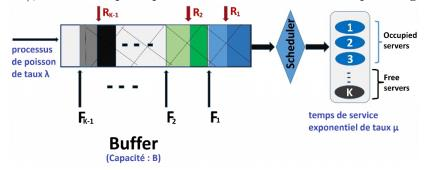
\includegraphics[width=0.70 \textwidth]{photo/modele_vm.jpg}
\caption{le data center avec une file d'attente multi serveur et avec une politique à seuils.}
\label{fig:graphe}
\end{figure}
\\
\noindent Comme le modèle de machines virtuelles décrit par la figure ci dessus,il nous propose que les clients arrivent dans la file d’attente multi-serveur (nous considère que 3 serveurs, 6 serveurs et 12 serveurs à l’évoluation dans la partie de l’étude experimentale), et les serveurs sont activés selon l’occupation du système. Au départ, un seul serveur était activé, puis quand le nombre de clients dépassera $F_{1}$, on activera un deuxième serveur, et jusqu’au seuil $R_{k}-1$ pour activer le k-ème serveur à la fois des désactivation des seuils $R_{1}$, ..., $R_{k}$-1.
\\
\noindent Autrement dit, on contôle le nombre de clients. S’ils dépassent de $R_{1}$ (ou $F_{1}$) on désactive le deuxième serveur, et donc un seul serveur est toujours activé. 
\\
\noindent Dans notre modèle, on définie qu’au départ des processus avec chacune en temps d’inter-arrivée Exponentielles $\frac{1}{\lambda}$ et ceux en temps de service Exponentiel de moyeene $\frac{1}{\mu}$.


\subsection{Chaîne de Markov}

\begin{tikzpicture}[auto,node distance = 2mm,start chain = going right,state/.append style = {thick,  minimum width=2.8em,text width=2.5em,align=center,on chain,fill=red, draw=none,text=black
 },
]

\node (s0)[state]    {$1$};   
\node (s1)[state]    {$2$};  
\node (s2)[state]    {$3$};  
\node (s3)[state]    {$F_{1}-1$};  
\node (s4)[state]    {$F_{1}$};     
\node (s5)[state]    {$r-1$}; 
\node (s6)[state]    {$r$}; 
\node (s7)[state]    {$B-1$}; 
\node (s8)[state]    {$B$}; 

\draw[->] (s0) edge[bend left] node (a1) {$\lambda$} (s1)
          (s1) edge[bend left] node (b1) {$\mu$} (s0)
          (s1) edge[bend left] node (a2) {$\lambda$} (s2)
          (s2) edge[bend left] node (b2) {$\mu$} (s1)
          (s3) edge[bend left] node (a3) {$\lambda$} (s4)
          (s4) edge[bend left] node (b3) {2*$\mu$} (s3);
\node[node distance=0.005cm,right=of s2] {$\bullet$ }; 

\draw[->] (s5) edge[bend left] node (a4) {$\lambda$} (s6)
          (s6) edge[bend left] node (b4) {$r$*$\mu$} (s5);
\node[node distance=0.005cm,right=of s4] {$\bullet$ }; 

\draw[->] (s7) edge[bend left] node (a5) {$\lambda$} (s8)
          (s8) edge[bend left] node (b5) {$r$*$\mu$} (s7);
\node[node distance=0.005cm,right=of s6] {$\bullet$ }; 
\end{tikzpicture}
\quad \\
\noindent La chaîne de Markov est une suite de variables aléatoires qui permet de faire la modélisation d’évolution dynamique d’un système aléatoire. On note {0 , 1 , 2 ... , F1-1 , F1 , F1+1 ... r-1 , r , r+1 ... , B-1 , B} la suite des instants de transition des états du système $\left \{X_{n},n\geq 0 \right \}$  dans notre suite. Et donc nous n’évoluons la distribution stationaire qu’au travers de la valeur actuelle. 
\quad \\
\noindent Notre modèle va créer et supprimer dynamiquement une machine virtuelle afin de faire l’évoluation. Nous develpons une fonction récursive pour obtenir les probabilités d’état stable du système. Et chaque probabilité est obtenu par la multiplication de P0 par la matrice A.
\quad \\
\noindent On calcule des versions successives de la distribution ainsi : 

\begin{equation}
    P_{i}= P_{0} *A_{i}
\end{equation}
\noindent  Et à chaque itération, ils respectent toujours: 
\begin{equation}
    \sum_{i=0}^{B} P_{i} *A_{i} = 1
\end{equation}

\noindent Quand considère à cette chaîne, on résume que :
\begin{enumerate}

\item 1 er seuil : $0\leq n\leq F_{1}-1$:
\begin{equation}
    A_{0} = 1 ; 
\end{equation}
\begin{equation}
    A_{1} = \left ( \frac{\lambda }{\mu }\right )^{1} ; \: ......
\end{equation}

\begin{equation}
    A_{F_{1}-1} = \left ( \frac{\lambda }{\mu }\right )^{F_{1}-1} ;
\end{equation}

\item 2 ème seuil : $F_{1}\leq n\leq F_{2}-1$:
\begin{equation}
    A_{F_{1}} = \left ( \frac{\lambda }{2*\mu }\right )^{1}\times A_{F_{1}-1} ;  
\end{equation}
\begin{equation}
    A_{F_{1}+1} = \left ( \frac{\lambda }{2*\mu }\right )^{2}\times A_{F_{1}-1} ; \: ......
\end{equation}
\begin{equation}
    A_{F_{2}-1} = \left ( \frac{\lambda }{\mu }\right )^{F_{2}-1-(F_{1}-1)}\times A_{F_{1}-1} ;
\end{equation}
......
\item n ème seuil (n est égal au nombre des serveurs): $F_{r}\leq n\leq F_{B}$:
\begin{equation}
    A_{F_{r}} = \left ( \frac{\lambda }{r*\mu }\right )^{1}\times A_{F_{r-1}-1} ; \: ......
\end{equation}
\begin{equation}
    A_{F_{B-1}} = \left ( \frac{\lambda }{r*\mu }\right)^{F_{B-1}-1-(F_{r}-1)}\times A_{F_{r-1}-1} ;
\end{equation}
\begin{equation}
    A_{F_{B}} = \left ( \frac{\lambda }{r*\mu }\right)^{F_{B}-1-(F_{r}-1)}\times A_{F_{r-1}-1} ;
\end{equation}
\end{enumerate}


\subsection{Algorithmique de calculer $A_{0}$...$A_{B}$}

\noindent Pour initialiser la matrice des seuils, on mise la distribution du nombre des états dans chacune. Et la capacité de file d'attente est initialisé à B. Dans ce cas là, si nous enregistrons tous les états de 0 à B , le nombre total des éléments posés dans la matrice est égal à B+1 (états). 
\quad \\
\noindent L’algorithme qu’on aurait dût implémenter est le suivant :
\begin{algorithm}
\caption{Calculer des valeurs de $A_{0}$...$A_{B}$}


\label{alg:Calculer des valeurs de A}
\begin{algorithmic}
\STATE {$function mat\left [ \right ] = Calculer\:A(index,\lambda,\mu\:tmp,pre)\{$} 
\STATE set $i=1$ 
\STATE set $tmp=0$ 

\REPEAT 
\IF {$index < Nb\:serveur$}
\IF {$index == 0$}
\FOR{$i=1$ to $seuils[index]$}
\STATE $tmp=\left ( \frac{\lambda }{\mu }\right )^{i-1-0}\times pre;$ 
\STATE $sum\:A=sum\:A + tmp;$ 
\STATE $mat\:A[]=ajout\:matrice(mat,tmp,pos+i-1);$ 
\ENDFOR

\ELSE
\FOR{$i=1$ to $seuils[index]$}
\STATE $tmp=\left ( \frac{\lambda }{\mu }\right )^{seuils[index-1]+i-1)-(seuils[index-1]-1)}\times pre;$ 
\STATE $sum\:A=sum\:A + tmp;$ 
\STATE $mat\:A[]=ajout\:matrice(mat,tmp,pos+i-1);$ 
\ENDFOR
\ENDIF

\STATE $pos = pos+seuils[index];$ 
\STATE $pre = tmp;$ 
\STATE $index++;$ 
\STATE $Calculer\:A(index,\lambda,\mu\:tmp + \mu,pre);$ 



\ELSE
\STATE $P_{0}=\frac{1}{sum\:A};$
\STATE $return\:\: mat\:A[];$
\ENDIF

\UNTIL{$index < Nb\:serveur$ }\\\}
\end{algorithmic}
\end{algorithm}

\subsection{Les formules d'analyser le système}
\noindent En fonction du nombre total de VMs, de la capacité du système et des seuils, nous analysons notre système avec des résultats calculés par l'algorithmique . Pour se faire: 
\begin{enumerate}
\item Calculer $P_{0}$ :
\begin{equation}
P_{0} + P_{1} + ... + P_{F_{1}-1} + P_{F_{1}} + ... P_{B} = 1
\end{equation} \\
\begin{equation}
P_{0} \times \left (  A_{0} + A_{1} + ... + A_{F_{1}-1} + A_{F_{1}} + ... A_{B} \right ) = 1 
\end{equation}\\
\begin{equation}
P_{0}=\frac{1}{\sum_{i=0}^{B} A_{i}}
\end{equation}

\item Probabilit\'e de blocage est égale à la probabilité qui se trouve dans l'état B:
\begin{equation}
    Pr = 1-\sum_{i=0}^{B-1}P_{i} = P_{B} = \left ( \frac{\lambda}{\mu}\right )^{B-1-\left ( r-1\right )}\times \cdot \cdot \cdot  \left ( \frac{\lambda}{\mu}\right )^{F_{2}-1-\left ( F_{1}-1\right )}\times \left ( \frac{\lambda}{\mu}\right )^{F_{1}-1}\times P_{0}
\end{equation}
\item Nombre moyen de requêts :
\citep{adams2015hitchhiker}
\begin{equation}
Nb\: moyen\: de\: requetes =\sum_{i=0}^{B}\left (i \times P_{i} \right ) 
\end{equation} 

\item Nous considèrons que la distribution selon des probabilités à chaque VM comme par exemple (6 clients arrivent dans 3 VMs):

\begin{center}
\begin{tabular}{ |c|c|c| } 
 \hline
 VM1 & VM2 & VM3 \\ 
 \hline
 2 états & 3 états & 2 états\\
 \hline
 $1 \times P_{0} + 1 \times P_{1} $&$ 2 \times P_{2} + 2 \times P_{3}+ 2 \times P_{4}$ & $ 3 \times P_{5}+3 \times P_{6}$ \\ 
 \hline
\end{tabular}
\end{center}

\noindent Nombre de machine virtuelles en fonctionnement :
\begin{equation}
Nb\:de\: vm = \sum_{i=1}^{nb\: de\: serveurs}\left (i\times \sum_{j=F_{\kappa}}^{F_{\kappa +1}-1}P_{j} \right )
\end{equation}
\noindent  ( Chaque VM fait lancer dans l’intervalle de état : $\left [ F_{\kappa},F_{\kappa +1}-1 \right ]$. )
\end{enumerate}

















 




\section{Etude Exp\'erimentale avec des diff\'erentes paramètres}
\newtheorem{theo}{th\'eor\`eme: }
\newtheorem{defe}{d\'efinition:}
\newtheorem{forule}{}

\noindent Pour nos expérimentations nous nous sommes concentrés sur les 3 modèles (avec des différents taux de service mais $\mu$=5 requêtes/h) suivant : \begin{itemize}
    \item modèle A (12 VMs de 1 coeur avec chacune un taux de service $\mu$) 
    \item modèle B (6 VMs de 2 coeur avec chacune un taux de service 2*$\mu$)
    \item modèle C (3 VMs de 4 coeur avec chacune un taux de service 4*$\mu$) \\
\end{itemize}


\noindent On a  également réalisé nos test avec différentes valeurs pour $\lambda$ : \begin{itemize}
    \item 50
    \item 60
    \item 70
    \item 80 
    \item 90
    \item 100\\
\end{itemize}

\noindent On définie que la capacité du système B est égal à 100.

\noindent Et enfin on l'a simulé sur la grande période à laquelle on l'effectue et attend son statut stable. Et après, on compare les résultats afin de déterminer la plus optimale.

\subsection{Résultats}
\subsubsection{Tableaux de performances}

\vspace{1cm}
\quad \\
\begin{tabular}{|c|c|c|c|c|}
\hline
\multicolumn{3}{|c}{modèle C : 3 MV} &\multicolumn{1}{c}{$\mu=20$}&\\
\hline 
\multicolumn{1}{|c|}{lambda}& \multicolumn{1}{c|}{resultat} & \multicolumn{1}{c|}{Pr blocage} & \multicolumn{1}{c|}{nbr requetes} & \multicolumn{1}{c|}{nbr MVs}  \\
\hline
 \multirow{2}{*}{$\lambda = 50$} & simulation & 0.0004011 & 61.7 & 2.236 \\ \cline{2-5}
                            & analytique & 0.0001695 & 65.97 & 2.4995 \\
                            \hline
  \multirow{2}{*}{$\lambda = 60$} & simulation & 0.01112 & 72.39 & 2.654 \\ \cline{2-5}
                            & analytique & 0.0263157 & 81.42056 & 2.92105 \\ \hline
  \multirow{2}{*}{$\lambda = 70$} & simulation & 0.1316 & 92.81 & 2.982 \\ \cline{2-5}
                            & analytique & 0.1432906 & 94.113288 & 2.998482 \\ \hline
  \multirow{2}{*}{$\lambda = 80$} & simulation & 0.2394 & 96.56 & 2.997 \\ \cline{2-5}
                            & analytique & 0.25 & 97.000784 & 2.999979 \\ \hline
  \multirow{2}{*}{$\lambda = 90$} & simulation & 0.3235 & 97.75 & 2.998 \\ \cline{2-5}
                            & analytique & 0.33333 & 98.00001 & 2.9999999 \\ \hline
  \multirow{2}{*}{$\lambda = 100$} & simulation & 0.3917 & 98.33 & 2.998 \\ \cline{2-5}
                            & analytique & 0.4 & 98.5 & 2.99999999 \\ \hline
\end{tabular}  

\vspace{1cm} \quad \\
\begin{tabular}{|c|c|c|c|c|}
\hline
\multicolumn{3}{|c}{modèle C : 6 MV} &\multicolumn{1}{c}{$\mu=10$}&\\
\hline 
\multicolumn{1}{|c|}{lambda}& \multicolumn{1}{c|}{resultat} & \multicolumn{1}{c|}{Pr blocage} & \multicolumn{1}{c|}{nbr requetes} & \multicolumn{1}{c|}{nbr MVs}  \\
\hline
 \multirow{2}{*}{$\lambda = 50$}  & simulation & 0 & 59.94 & 4.243 \\ \cline{2-5}
                            & analytique & 0.000841 & 71.6329 & 4.99579 \\ \hline
                            
  \multirow{2}{*}{$\lambda = 60$} & simulation & 0.002463 & 72.8 & 5.036 \\ \cline{2-5}
                            & analytique & 0.03726 & 86.634695 & 5.776433 \\ \hline
  \multirow{2}{*}{$\lambda = 70$}  & simulation & 0.09933 & 88.66 & 5.726 \\ \cline{2-5}
                            & analytique & 0.145723 & 94.491871 & 5.9799 \\ \hline
  \multirow{2}{*}{$\lambda = 80$}  & simulation & 0.2401 & 96.34 & 5.969 \\ \cline{2-5}
                            & analytique & 0.250198 & 97.018786 & 5.99841 \\ \hline
  \multirow{2}{*}{$\lambda = 90$}& simulation & 0.3307 & 97.82 & 5.99 \\ \cline{2-5}
                            & analytique & 0.33335 & 98.001165 & 5.999849 \\ \hline
  \multirow{2}{*}{$\lambda = 100$} & simulation & 0.3973 & 98.29 & 5.992 \\ \cline{2-5}
                            & analytique & 0.4 & 98.500101 & 5.99998 \\ \hline
\end{tabular}  
\vspace{1cm}  \quad \\
\begin{tabular}{|c|c|c|c|c|}
\hline
\multicolumn{3}{|c}{modèle C : 12 MV} &\multicolumn{1}{c}{$\mu=5$}&\\
\hline 
\multicolumn{1}{|c|}{lambda}& \multicolumn{1}{c|}{resultat} & \multicolumn{1}{c|}{Pr blocage} & \multicolumn{1}{c|}{nbr requetes} & \multicolumn{1}{c|}{nbr MVs}  \\
\hline
 \multirow{2}{*}{$\lambda = 50$}& simulation & 0 & 45 & 6.37 \\ \cline{2-5}
                            & analytique & 0.001881 & 75.48 & 9.98 \\ \hline
  \multirow{2}{*}{$\lambda = 60$}  & simulation & 0 & 53.4 & 7.457 \\ \cline{2-5}
                            & analytique & 0.0459 & 88.83 & 11.44 \\ \hline
  \multirow{2}{*}{$\lambda = 70$}  & simulation & 0 & 66.85 & 9.068 \\ \cline{2-5}
                            & analytique & 0.15 & 94.91 & 11.89 \\ \hline
  \multirow{2}{*}{$\lambda = 80$} & simulation & 0.0369 & 76.24 & 10.03 \\ \cline{2-5}
                            & analytique & 0.25 & 97.08 & 11.98 \\ \hline
  \multirow{2}{*}{$\lambda = 90$} & simulation & 0.2254 & 90.81 & 11.23 \\ \cline{2-5}
                            & analytique & 0.3335 & 98.011 & 11.995 \\ \hline
  \multirow{2}{*}{$\lambda = 100$} & simulation & 0.3562 & 96.09 & 11.72 \\ \cline{2-5}
                            & analytique & 0.40005 & 98.50 & 11.998 \\ \hline
\end{tabular}  

\begin{comment}
\subsubsection{Analyses}
On observe que globalement l'accélération est efficace pour une période allant de 10 à 20. En revanche il faut noter que l'effet est positif seulement lorsque $\alpha$ est proche de 1. Ainsi dans nos experimentations les améliorations se font surtout dans le cas où $\alpha$ = 0.95.
\\

En général on observe un gain qui va jusqu'à 14\% (cas du graphe de l'Inde avec une période de 10). En revanche il semble que certaines topologies se prêtent très mal à cet algorithme, par exemple plus la période est basse pour le graphe de Stanford et plus la convergence est lente. On observe même une absence de convergence quand la période est de 5. Globalement il semble qu'une période trop petite soit très risquée : il semble plus rentable d'augmenter la période d'accélération pour réduire le temps(sec) moyen de calcul.
\end{comment}
%\newpage

\subsection{Analyses de graphes}
\begin{figure}[ht!]
\centering
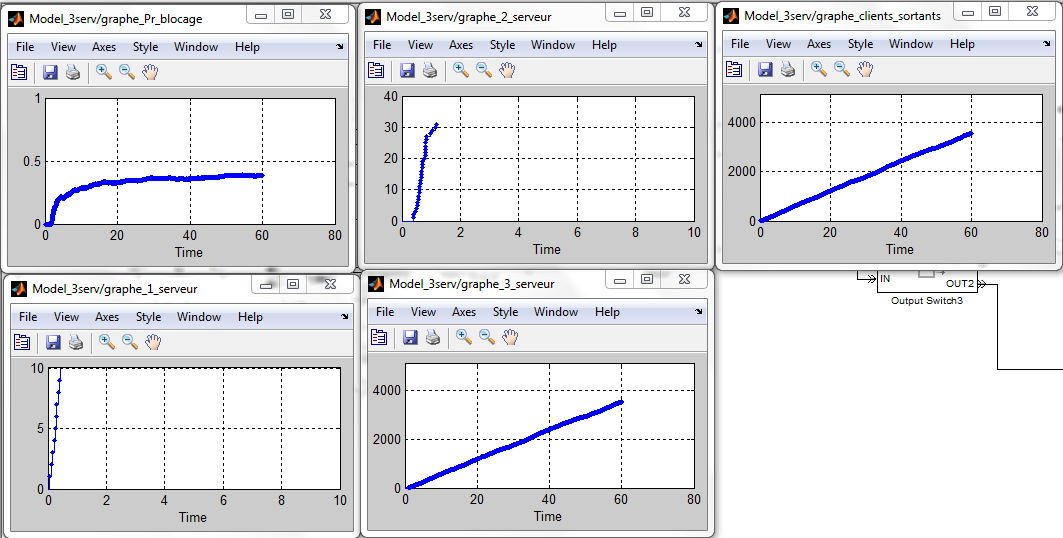
\includegraphics[width=0.95 \textwidth]{photo/graphe_model_3MV.png}
\caption{Les graphes de simulation avec 3 MVs et le paramètre $\lambda$=100}
\label{fig:graphe1}
\end{figure}
\newpage
\noindent Ces graphes représentent les résultats de la simulation du Modèle C avec les paramètres suivants: 3VM, Taux d’arrivées  $\lambda$=100, Taux de service  4$\mu$ ( $\mu$=5 requêtes/h) et la Capacité du système B=100.

Nous obtenons 5 graphes (graphe de: probabilité de blocage, les clients(ou taches) passé par un serveur, les clients passé par deux serveurs, les clients passés par trois serveurs et les client passé par le système) en prenant un temps réduit de la simulation (60) pour avoir des graphes lisibles.

"graphe$\_$Pr$\_$blocage" c'est le graphe de probabilité de blocage qui montre que dans les premiers temps un blocage nul cela indique que tous les clients arrivés sont bien servis. Dès que la courbe dépasse la valeur 0, tous les serveurs sont activé car on a utilisé la distribution exponentielle pour générer des clients (le taux d'arrivées augmente selon la loi exponentielle), on remarque une augmentation progressive de la probabilité de blocage par rapport au temps car le taux d'arrivées est toujours en augmentation. au temps supérieur à 20 la courbe devient presque stable.

"graphe$\_$1$\_$serveur"," graphe$\_$2$\_$serveur ", "graphe$\_$3$\_$serveur" sont des graphes représentant le nombre de clients servis par 1, 2 ou 3 serveurs par rapport au temps. "graphe$\_$1$\_$serveur" montre que dans les premiers temps les clients sont servis par un seul serveur.

"graphe$\_$2$\_$serveur " commence après que le "graphe$\_$1$\_$serveur" atteint son seuil et qu'il a traité certains clients.

"graphe$\_$3$\_$serveur" commence quand le "graphe$\_$2$\_$serveur " atteint son seuil et  il continu à augmenter jusqu'à la fin de la simulation.

"graphe$\_$client$\_$sortants" ce graphe montre que tous les clients sont servis par le système, on remarque qu'il a la même allure que le "graphe$\_$3$\_$serveur". cela indique que les clients servis par ce système sont presque tous traités par les 3 serveurs  avec une probabilité de blocage due à un Taux d’arrivées plus élevé par rapport à la capacité de système.
\\
\newpage
\begin{figure}[ht!]
\centering
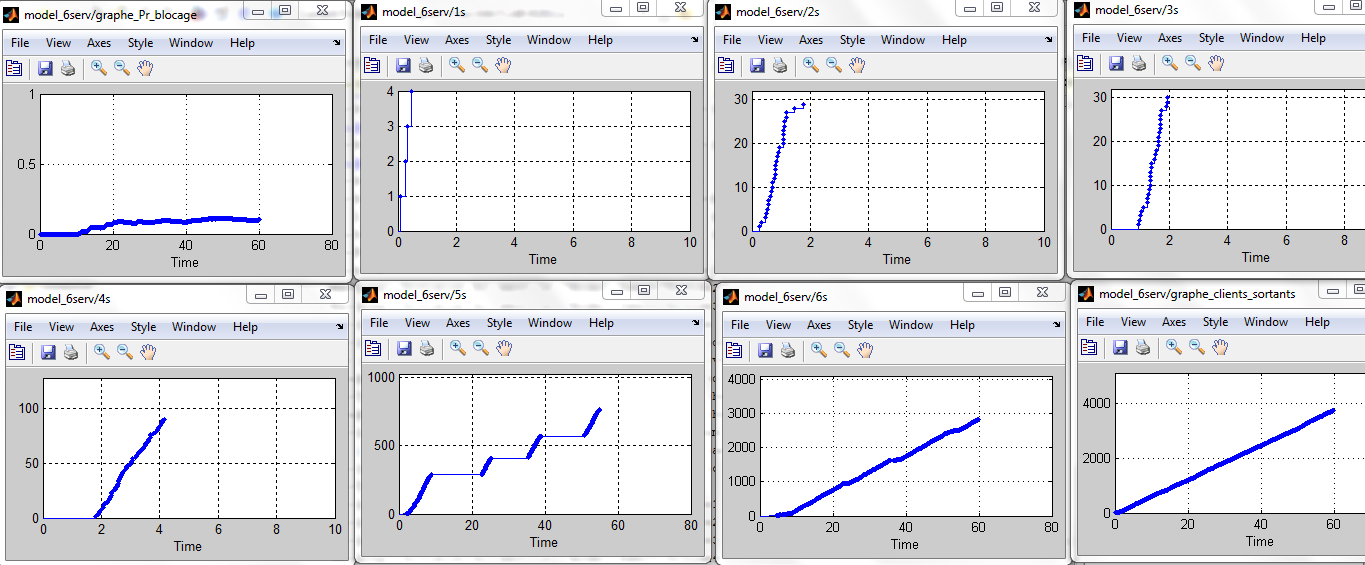
\includegraphics[width=0.95 \textwidth]{photo/graphe_6MV.png}
\caption{Les graphes de simulation avec 6 MVs et le paramètre $\lambda$=70}
\label{fig:graphe2}
\end{figure}
\noindent Ces graphes représentent les résultats de la simulation du Modèle B avec les paramètres suivants: 6VM, Taux d’arrivées  $\lambda$=70, Taux de service  2$\mu$($\mu$=5 requêtes/h) et la Capacité du système B=100.

\noindent Dans ce modèle on constate que le fonctionnement des serveur est similaire au fonctionnement des serveurs du modèle précédant (à chaque déplacement de seuil d'un serveur, le prochain  serveur se lance), le graphe "5s" montre que le les 5 serveurs fonctionnent de manière discontinue, cette discontinuité est due au déplacement de leur seuil ce qui entraine le fonctionnement avec 6 serveurs, lorsque le taux d'arrives est inferieur au seuil des 5 serveurs, le sixième serveur sera désactivé (fonctionnement en 5 serveurs).   

\noindent On observe que la probabilité de blocage a diminué par rapport au modèle précédant car on a simuler avec un taux d'arrivés  réduit
 \newpage
 \begin{figure}[ht!]
\centering
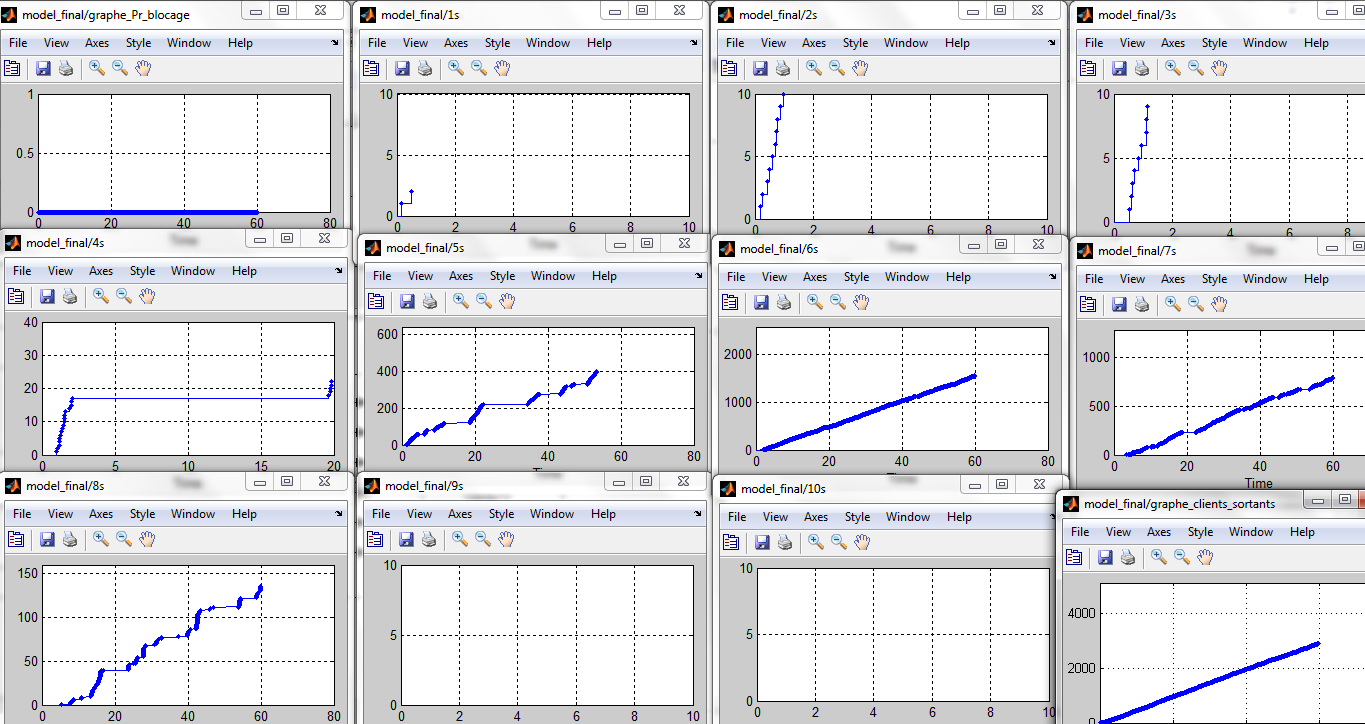
\includegraphics[width=0.95 \textwidth]{photo/graphe_12MV.png}
\caption{Les graphes de simulation avec 12 MVs et le paramètre $\lambda$=50}
\label{fig:graphe3}
\end{figure}
\noindent Ces graphes représentent les résultats de la simulation du Modèle A, avec les paramètres suivants: 12VM, Taux d’arrivées  $\lambda$=50, Taux de service  $\mu$=5 requêtes/h et la Capacité du système B=100.

Dans ce modèle on voie le même principe de fonctionnement des serveurs comme les modèles précédents. de plus, il n'existe aucune courbe sur les graphes "9s", "10s", "11s" et "12s" car le taux d'arrivées n'a pas dépasser le seuil de "8s" de ce fait, la probabilité de blocage est toujours nulle comme le montre le graphe"graphe$\_$Pr$\_$blocage".


 




\section{Difficuli\'es rencontr\'ees}

\subsection{Résultats de simulation et de programmation}

\noindent 
les resultats obtenu par la simulation de notre modèle sont tres proche des resultats de la progmmation. Néanmoins nous avons rencontré plusieurs obstacles. Principalement, la probabilité de blocage a une marge d'erreur de l'ordre de $ 10^{-2} $. Parfois les valeurs de nombre moyen de requêtes sont différentes lorsque $\lambda$ est petit.
les valeurs de sorties sont affichées, montrant qu'il y a des clients perdus dans notre système (ce sont pas des clients bloqués.). 
\\
\noindent Nous avons donc ignoré ces erreurs après une discussion avec notre professeur et nous considèrons que le programmation nous donne des résultats idéals sans perte pendant le traitement des serveurs.

\section{Conclusion}
\noindent Nous avons proposé une implémentation en C de l’algorithme de simulation de machine virtuelle selon la propriété de la distribution stationnaire. 
\\
\noindent Pour avoir les résultats les plus performants, on a proposé trois modèles de simulation avec des différentes configurations, les VMs sont saturées lorsque le Taux d'arrivées ($\lambda$) dépasse leurs seuils et la probabilité de blocage augmente aussi quand $\lambda$ continu à augmenter après avoir déjà dépassé la capacité du système.

\noindent Après plusieurs simulations, nous avons trouvé que la performance du VM en modèle A (12 serveurs) est la plus efficace par rapport au modèle C (3 serveurs) et au modèle B (6 serveurs) car le cas de blocage en modèle A apparaît lorsque $\lambda$ = 70, en modèle B quand  $\lambda$ = 60 et en modèle C quand $\lambda$ = 50.

\noindent Nos résultats de simulation correspondent avec les résultats obtenus dans l'article présenté par V.Goswami, S.S.Patra G.B.Mund.


\bibliographystyle{plain}
\bibliography{references}

\end{document}
